\documentclass{article}
\usepackage{graphicx} % Required for inserting images
\usepackage{amsmath}
\usepackage{indentfirst}

\title{BI-ZUM ULOHA 2}
\author{Maksym Khavil}
\date{March 2025}

\begin{document}

\maketitle
\newpage
\section{}

Nasledující dva obraykz ukazujou běh Greedz search a Dijkstra na nášem grafu. Žlutě jsou podtrhntuté otevřené vrcholy, pod ními je napsána vzdalenost od Mahadia. Vpravo je pořadek uzavření vrcholů.

\begin{figure}[h]
    \centering
    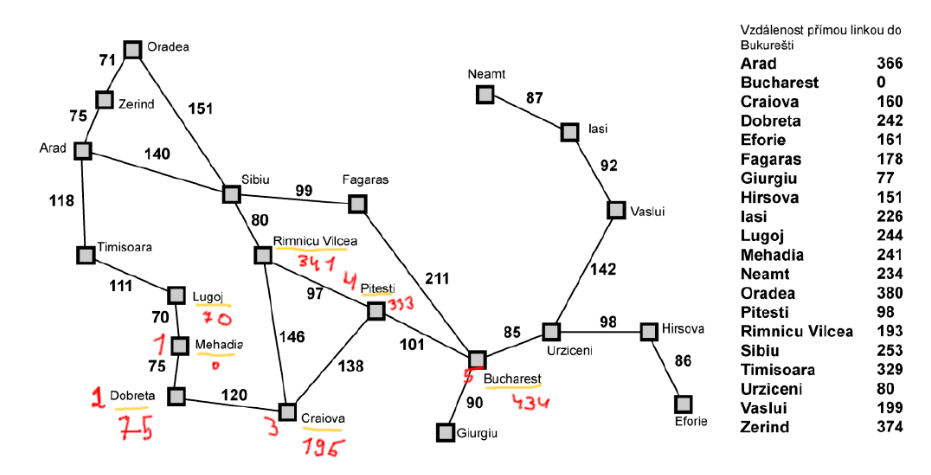
\includegraphics[width=\linewidth]{zum-greeedy.png}
    \caption{Průběh Greedy BFS}
    \label{fig:sample}
\end{figure}
\begin{figure}[h]
    \centering
    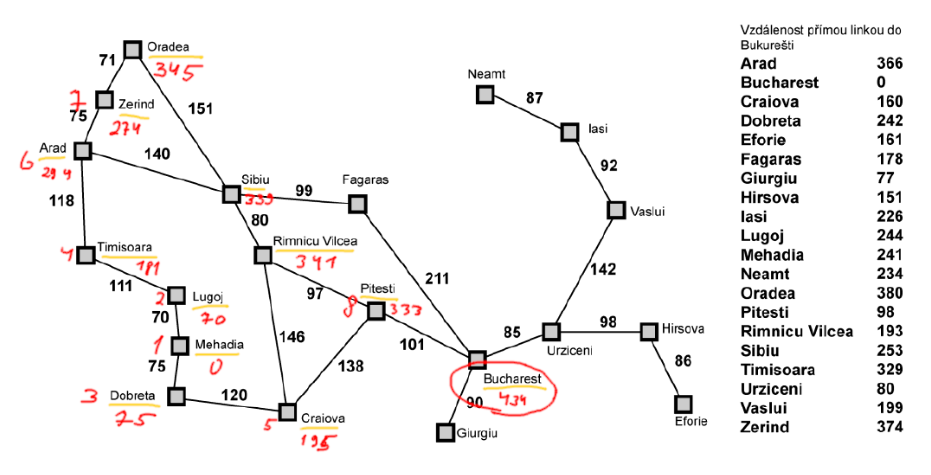
\includegraphics[width=\linewidth]{zum-dijkstra.png}
    \caption{Průběh Dijkstra}
    \label{fig:sample}
\end{figure}

\newpage
\section{}

Robot se pohybuje po mřížce, proto aby se dostal do jakékoliv cíle musí udělat $K$ kroku. Počet kroku robotu je větší nebo rovné než manhattenovská vzdalenost, protože má projít vertikálně a vodorovně, tj manhattenovská vzdalenost je přípustá. Taxicab distance je větší než euklidovská distance, proto je také přípustna. Heuristika pohazející se z druhé mocniné euklidové vzdaleností nemusí byt připustná. Pro cestu 10 vpravo 1 nahoru tato vzdalenost vratí 101, což je vyrazně víc než de facto cena 11.

Pro řešení problemu nejvhodnější bude taxicab distance, protože je připustná a dominuje euklidovskou vzdalenost.

\newpage
\section{}

\subsection{Každá konzistentní heuristika je přípustná}

Nechťme $h:S\rightarrow R$ je  heuristika na grafu $G=(S, A)$ a je konzistentní ($c(n,m)$ je cena cesty z $n$ do $m$):

\begin{equation*}
    \forall n,m \in S: h(n) \leq c(n, m) + h(m)
\end{equation*}

Nechťme $h^*$ je optimální heuristika a platí $h^*(n) = c(n, T)$, kde $T$ je cílový stav. Dosazením $m = T$ do rovnice nahoře dostaváme:

\begin{equation*}
    h(n) \leq c(n, T) + h(T) \leq h^*(n) + 0 = h^*(n)
\end{equation*}

\subsection{Přípustná nekonzistentní heuristika}

Na nasledhujícím grafu $S$ je počateční stav a $T$ je cílový stav platí

\begin{equation*}
    h(S) > c(S, a) + h(a)= 3 + 0.5
\end{equation*}

Tedy tato heuristika není konzistentní, ale je přípustná.

\begin{figure}[h]
    \centering
    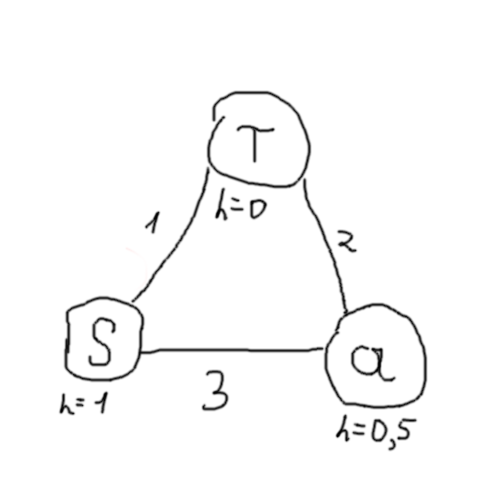
\includegraphics[scale=1]{zum-cexample.png}
    \caption{}
    \label{fig:sample}
\end{figure}

\end{document}
